\documentclass[12pt, a4paper]{article}
\setlength{\textheight}{24cm}
\setlength{\textwidth}{16cm}
\setlength{\topmargin}{0cm}
\setlength{\evensidemargin}{0cm}
\setlength{\oddsidemargin}{0cm}
\usepackage[affil-it]{authblk}
\usepackage{graphics}
\usepackage{graphicx}
\usepackage{caption}
\usepackage{float}
\usepackage[british]{babel}
\usepackage{hyperref}
\usepackage{subcaption}
\date{}
\begin{document}
\title{Comparison of Several Frameworks for General-Purpose Programming and the  Computation of FFTs on GPUs}
\author{Philippe Gambron \thanks{\texttt{philippe.gambron{@}stfc.ac.uk}}, Sue Thorne \thanks{\texttt{sue.thorne{@}stfc.ac.uk}}}
\affil{Science and Technology Facilities Council, Hartree Centre, Rutherford Appleton Laboratory, Harwell Campus, Harwell Oxford, OX11 0QZ, United Kingdom}
\maketitle
\begin{abstract}
We compare the performance of several frameworks that can be used, in C, for general-purpose programming on a graphical processing unit or to compute Fast Fourier Transforms.  
\end{abstract}
\section{Introduction}
For a bit more than a decade, the use of graphical processing units (GPU) has become increasingly widespread. They are indeed capable of significantly increasing the performance of a single workstation or compute node. While there are some overheads associated to the data transfers with the memory and some constraints on the types of algorithms can be efficiently programmed, one can obtain tremendous performance gains on suitable problems.\\

In this report, we will compare the performances obtained with several of these frameworks.  We measured them using a simple general-purpose programming example and by computing Fast Fourier Transforms (FFT) on the GPU by using the libraries provided by these frameworks. 

\section{Overview of the chosen libraries}
We consider the following frameworks for GPU programming: CUDA \cite{cuda}, OpenCL \cite{opencl}, \mbox{OpenACC} \cite{openacc}, OpenMP \cite{openmp}\footnote{From version 4.0, OpenMP offers GPU programming.} and Kokkos \cite{kokkos}. The first three of these frameworks provide as well FFT libraries. Respectively, they are: cuFFT \cite{cufft}, clFFT \cite{clfft} and AccFFT \cite{accfft} (Table \ref{ffttable}). They can perform complex transforms, real-to-half-complex ones (and conversely) as well as, in the case of FFTW, real-to-real transforms when the signal is odd or even. The half-complex output consists in half as many complex values as there were points in the signal, taking advantage of the hermiticity of the Fourier transform of a real function.\\
\begin{table}[H]
\captionsetup{width=0.8\textwidth}
\centering
\begin{tabular}{|p{2.5cm}||p{2.5cm}|p{1cm}|p{3cm}|p{3cm}|p{2cm}|p{2cm}|}
\hline
& Type & Dim. & Radices & Licence \\
\hline
\hline
AccFFT & R$\to$H,\ \ \  C$\to$C& 3& & GPL v2\\
\hline
clFFT  &  R$\to$H,\ \ \  C$\to$C,\ \ \ \  H$\to$R& 1, 2, 3 & 2, 3, 5, 7 & Proprietary\\
\hline
cuFFT  &  R$\to$H,\ \ \  C$\to$C,\ \ \ \  H$\to$R & 1, 2, 3 & 2, 3, 5, 7 & GPL v3\\
\hline
\end{tabular}
\caption{Overview of the FFT libraries considered. R stands for real, C, for complex, and HC, for half-complex.}
\label{ffttable}
\end{table}
\section{Benchmark}
The benchmark\footnote{The source code is available at: \hyperlink{https://github.com/SoftwareOutlook/GPU}{https://github.com/SoftwareOutlook/GPU}.} consists in processing a real or complex signal on a domain in 1, 2 or 3 dimensions. We first multiply it by a series of real signals, thus producing another series of real or complex signals, and then take their FFT.  The purpose was to mimick a problem submitted to us by the CCP PET-MR collaboration \cite{ccppetmr}, within the Software Outlook initiative \cite{softwareoutlook}, who needed to multiply a complex image by a series of coil sensitivities and then compute the FFT of these products. In Section \ref{PRODUCT}, we benchmark the product while, in Section \ref{FFT}, we study the performance obtained while computing the FFT. For the example specific to the CCP/PET-MR collaboration (Section \ref{CCPPETMR}), we take the FFT of 32 square images. In the more general case, we use a single signal but consider domains in 1, 2 or 3 dimensions. The bemchmark is depicted in Fig. \ref{benchmark} and described more extensively in \cite{FFTREPORT}.\\

\begin{figure}[H]
\captionsetup{width=0.6\textwidth}
\centering
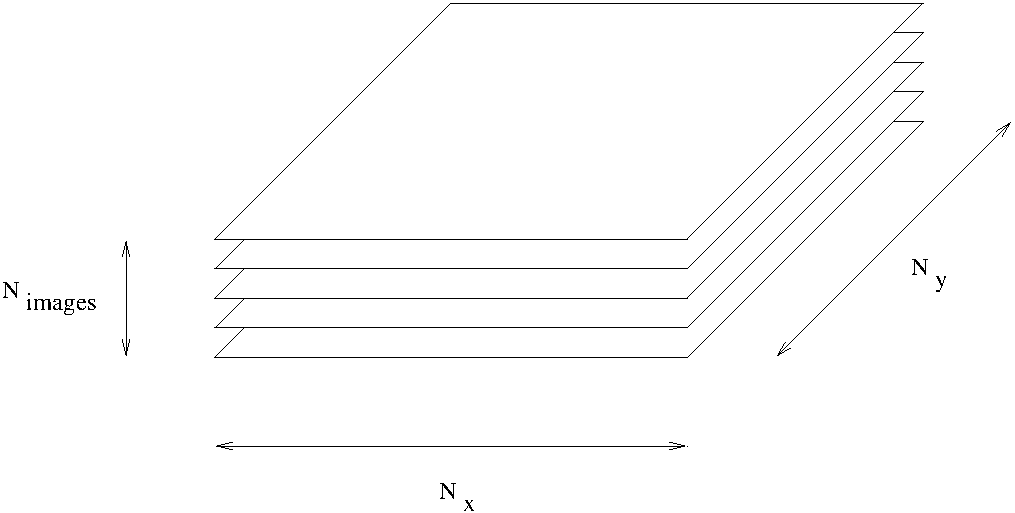
\includegraphics[height=5cm]{benchmark.pdf}
\caption{The benchmark consists in taking the FFT of several images. Each of them is made of real or complex values and can be a simple line, a rectangle or a cuboid.}
\label{benchmark}
\end{figure}

To study the performances achieved while computing the FFT in the general case, we use a number of points varying from $\sim 10^3$ to $\sim 10^8$, in 1, 2 or 3 dimensions (Sections \ref{PERFORMANCE1D}, \ref{PERFORMANCE2D} and \ref{PERFORMANCE3D} respectively). The domains have sides of equal lengths (square or cubic) or are flattened (rectangle or cuboid). These dimensions could be powers of 2, products of powers of small integers (2, 3, 5 and 7) or prime numbers. The values appearing in the graphs are the initialisation and execution times averaged over 10 runs. The bumps remaining on the graphs in some cases appear consistently when we repeat the measurements.

\section{Setup}

The measurements were carried out on a system featuring an Intel Xeon W-2133 CPU (6 cores, 3.6 GHz), a NVIDIA Quadro GV100 GPU and 12 GB of RAM. We used GCC (version 7.3.0) and the following frameworks: CUDA (version 10.0.130), OpenCL (version 1.2.7), OpenACC (version 2.7), OpenMP (version 4.0.0) and Kokkos (version 2.9.0) and clFFT (version 2.0). In this context, one disadvantage of OpenCL becomes apparent. The support for it is more limited. The most recent versions (from 2.0) are not completely supported by NVIDIA GPUs.  

\section{Product}\label{PRODUCT}
We first compare the multiplication of an array of $2^{24}$ real or complex numbers by an array of real numbers by considering the operation executed respecively in a serial way on the processor, in a multi-threaded way on the processor as well using OpenMP and Kokkos, on the GPU using CUDA, OpenCL, OpenACC, OpenMP and Kokkos. In the case of CUDA and OpenCL, we have made the comparison using streams or queues. This is a mechanism that allows the concurrent execution of kernels as well as overlapping data transfers in different directions.
\begin{figure}[H]
\captionsetup{width=0.8\linewidth}
\centering
\begin{subfigure}{.5\textwidth}
\centering
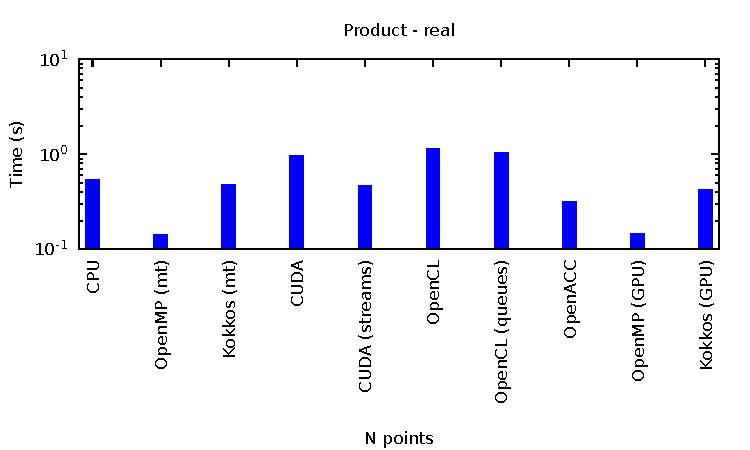
\includegraphics[width=.9\linewidth]{graphs/product-r.pdf}
\caption{Real}
\label{PRODR}
\end{subfigure}%
\begin{subfigure}{.5\textwidth}
\centering
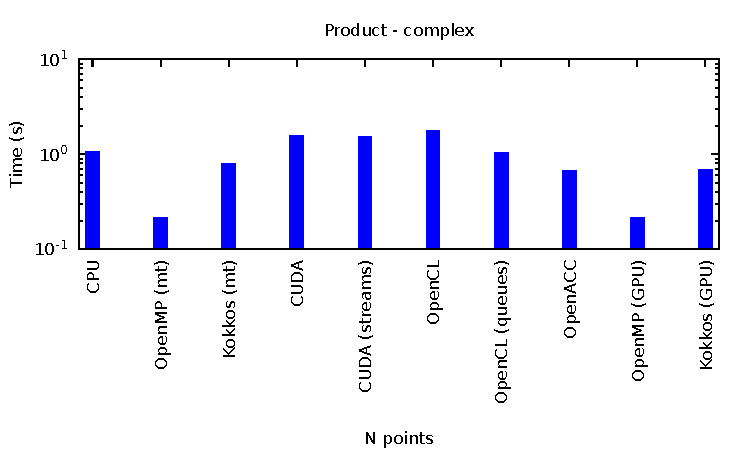
\includegraphics[width=.9\linewidth]{graphs/product-c.pdf}
\caption{Complex}
\label{PRODC}
\end{subfigure}
\caption{Execution time for the product of a large number of $2^{24}$ real and complex points using several frameworks.}
\label{1DFFTW}
\end{figure}

We observe that the best performance is obtanined with OpenMP, both on the CPU and the GPU. We noted that, while compiling the example involving Kokkos was straightforward, enabling CUDA required a compilation that was more complicated\footnote{An external makefile as well as a header file containing the configuration must be included. This will produce, during compilation, several object files in the current directory that will have to be linked to produce our executable file. See \cite{KOKKOSDOC} for details. The environment variable \texttt{OMP\_PROC\_BIND} had also to be set to \texttt{spread} before the execution of the program.}.
\section{Fast Fourier Transform}\label{FFT}
We repeat the analysis carried out in \cite{FFTREPORT}. We measure the initialisation and execution times obtained by computing the FFT transform with CUDA, OpenCL and OpenACC for signals that were real and complex in one, two and three dimensions. We initially consider domains whose sides are identical and that contain a number of points varying from $\sim 10^3$ to $\sim 10^8$. \\

Before we study in detail the performance obtained with GPUs, it is enlightening to illustrate the effect they can provide by comparing the performance obtained with CUDA with the one achieved with FFTW running in a serial way on the CPU. We have carried out these measurements by computing the FFT of real and complex signals, in one dimension. For a large number of points, the GPU improves the performance by almost an order of magnitude while it is slower for a small number of points because of the overheads (Figure \ref{COMPGPUCPU}).
\begin{figure}[H]
\captionsetup{width=0.8\linewidth}
\centering
\begin{subfigure}{.5\textwidth}
\centering
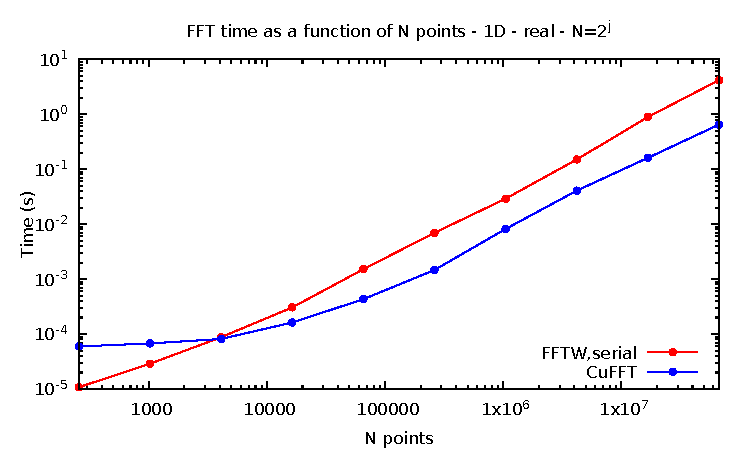
\includegraphics[width=.9\linewidth]{graphs/gpucpucomparison-r.pdf}
\caption{Real}
\label{PRODR}
\end{subfigure}%
\begin{subfigure}{.5\textwidth}
\centering
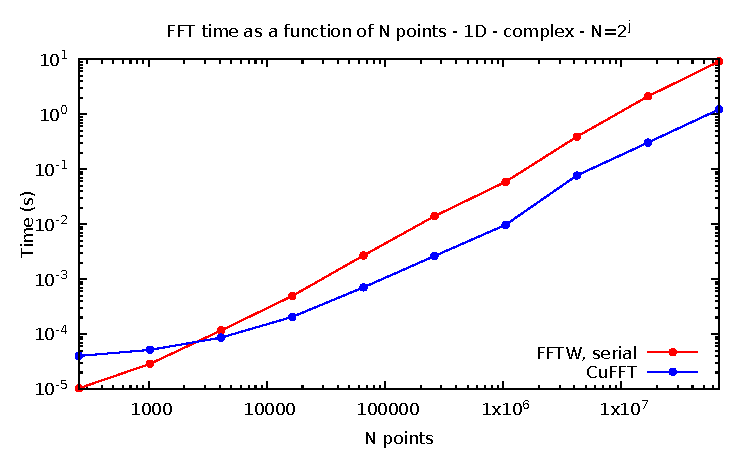
\includegraphics[width=.9\linewidth]{graphs/gpucpucomparison-c.pdf}
\caption{Complex}
\label{PRODC}
\end{subfigure}
\caption{Comparison between the execution times obtained with CUDA and FFTW running in a serial way on the CPU.}
\label{COMPGPUCPU}
\end{figure}


\subsection{Effect of the domain size in one dimension}\label{PERFORMANCE1D}
We compare the performance of these FFT libraries (Sections \ref{FFTCUDA1D}, \ref{FFTCL1D} and \ref{FFTACC1D}), in one dimension, for a real or complex signal consisting of numbers of points that are a power of 2, the product of powers of small integers (2, 3, 5 and 7) or prime numbers (Table \ref{1DSIZES}). We subsequently compare the libraries among themselves with powers of 2 (Section \ref{FFTPOW21D}) and in the general case (Section \ref{FFT1D}).\\ 
\begin{table}[H]
\centering
\begin{tabular}{|l|l|l|}
  \hline
  \multicolumn{3}{|c|}{$N_x$}\\
  \hline
  \hline
Powers of 2 & prod. pow. int. & primes\\ \hline
$2^8=256$ & $2\ 3\ 5\ 7 = 210$	& 257 \\ \hline
$2^{10}=1024$ & $2^2\ 3^2\ 5\ 7 = 1260$ & 1021 \\ \hline
$2^{12}=4096$ & $2^2\ 3^3\ 5\ 7 = 4410$ & 4093 \\ \hline
$2^{14}=16384$ & $2\ 3^2\ 5^3\ 7=15750$ & 16381 \\ \hline
$2^{16}=65536$ & $2\ 3^3\ 5^5\ 7^2 = 66150$ & 65521 \\ \hline
$2^{18}=262144$ & $2\ 3\ 5^3\ 7^3 = 257250$ & 262139 \\ \hline
$2^{20}=1048576$ & $2\ 3\ 5^2\ 7^4 = 1080450$ & 1048573 \\ \hline
$2^{22}=4194304$ & $2^3\ 3^2\ 5^2\ 7^4 = 4321800$ & 4194301 \\ \hline
$2^{24}=16777216$ & $2^3\ 3^2\ 5^4\ 7^3 = 15435000$ & 16777213 \\ \hline
$2^{26}=67108864$ & $2^3\ 3^3 5^3 7^4 = 64827000$ & 67108859 \\ \hline
\end{tabular}
\caption{Number of points used for the benchmark in one dimension}\label{1DSIZES}
\end{table}
The best performance is obtained with CUDA and, to a lesser extent, OpenCL. However the latter suffers from another drawback. While, with the two other frameworks, the initialisation time increases as a function of the domain size, it remains constant and quite large with OpenCL. It can be close and, in some cases, even larger than the execution time. We also observe that, for small numbers of points, the performance tends to be better for powers of 2, than for products of small integers and finally for prime numbers.
  
\begin{figure}[H]
\captionsetup{width=0.8\linewidth}
\centering
\begin{subfigure}{.5\textwidth}
\centering
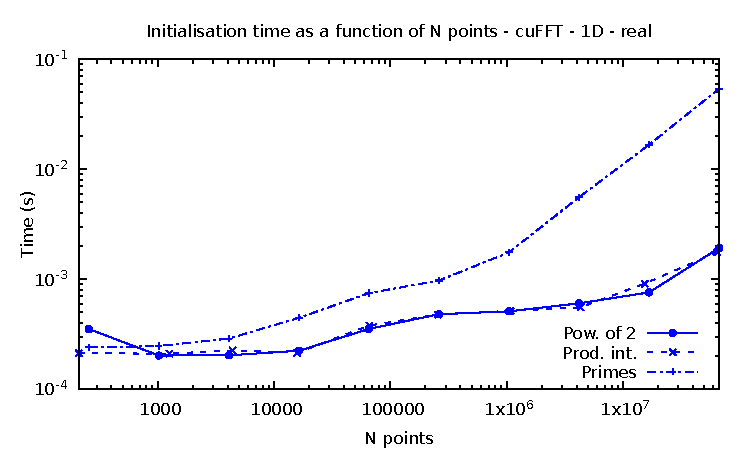
\includegraphics[width=.9\linewidth]{graphs/fft-cuda-1d-pow2-r-init.pdf}
\caption{Intialisation (real)}
\label{FFTCUDA1DRI}
\end{subfigure}%
\begin{subfigure}{.5\textwidth}
\centering
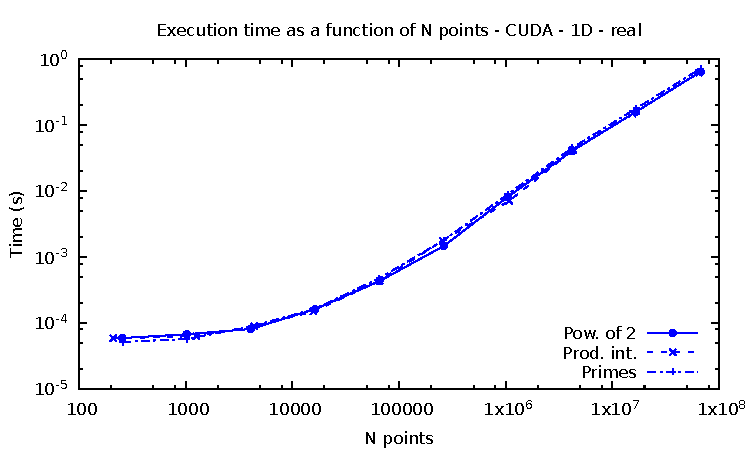
\includegraphics[width=.9\linewidth]{graphs/fft-cuda-1d-pow2-r-exec.pdf}
\caption{Execution (real)}
\label{FFTCUDA1DRE}
\end{subfigure}\\
\begin{subfigure}{.5\textwidth}
\centering
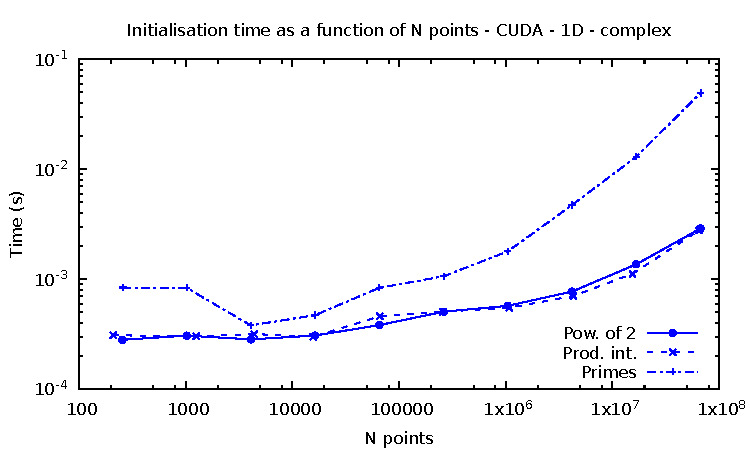
\includegraphics[width=.9\linewidth]{graphs/fft-cuda-1d-pow2-c-init.pdf}
\caption{Intialisation (complex)}
\label{FFTCUDA1DCI}
\end{subfigure}%
\begin{subfigure}{.5\textwidth}
\centering
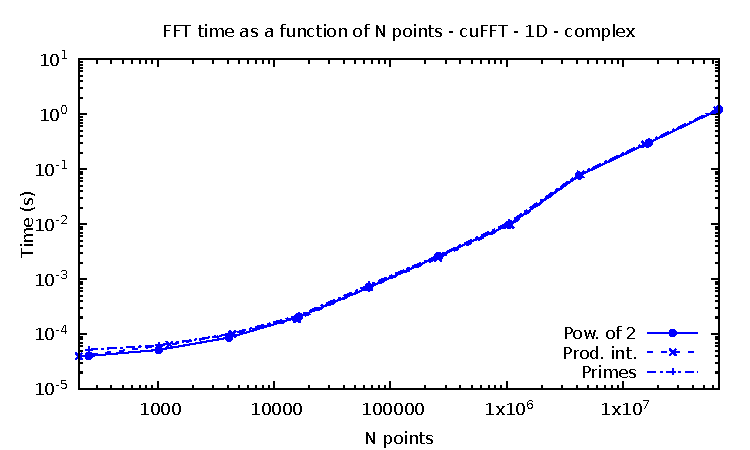
\includegraphics[width=.9\linewidth]{graphs/fft-cuda-1d-pow2-c-exec.pdf}
\caption{Execution (complex)}
\label{FFTCUDA1DCE}
\end{subfigure}
\caption{Initialisation and execution times as a function of the number of points (CUDA, 1 dimension)}
\label{FFTCUDA1D}
\end{figure}


\begin{figure}[H]
\captionsetup{width=0.8\linewidth}
\centering
\begin{subfigure}{.5\textwidth}
\centering
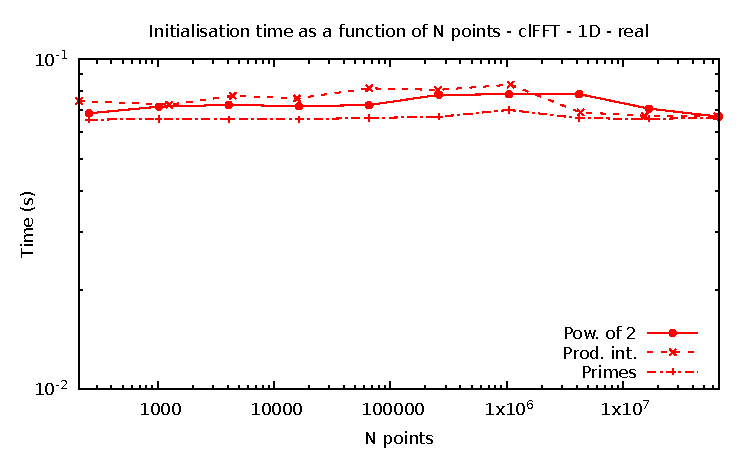
\includegraphics[width=.9\linewidth]{graphs/fft-opencl-1d-pow2-r-init.pdf}
\caption{Intialisation (real)}
\label{FFTCL1DRI}
\end{subfigure}%
\begin{subfigure}{.5\textwidth}
\centering
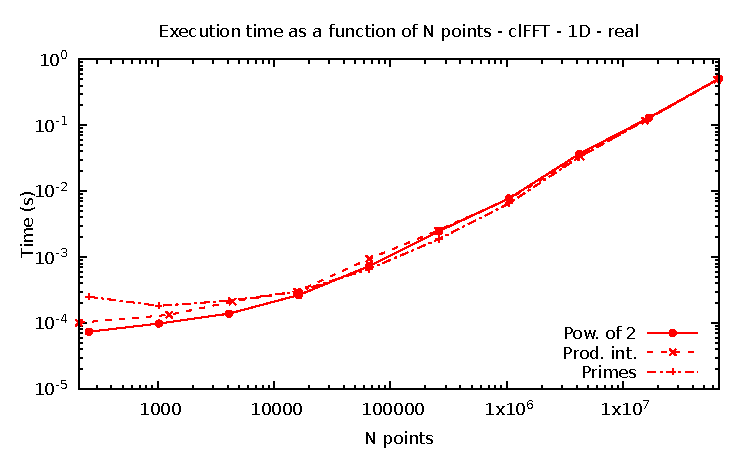
\includegraphics[width=.9\linewidth]{graphs/fft-opencl-1d-pow2-r-exec.pdf}
\caption{Execution (real)}
\label{FFTCL1DRE}
\end{subfigure}\\
\begin{subfigure}{.5\textwidth}
\centering
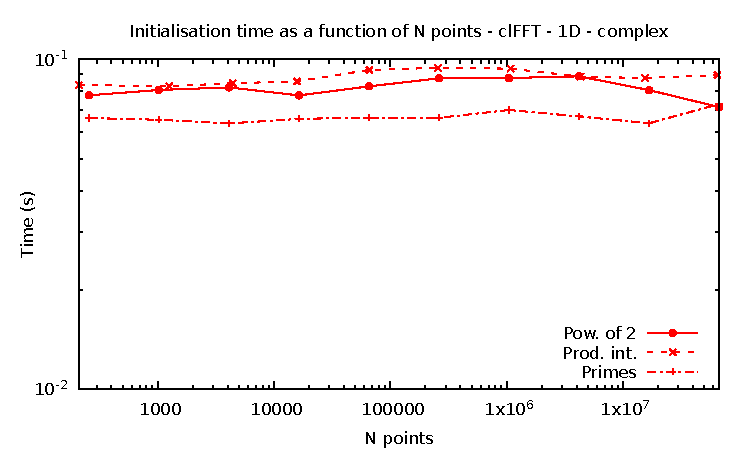
\includegraphics[width=.9\linewidth]{graphs/fft-opencl-1d-pow2-c-init.pdf}
\caption{Intialisation (complex)}
\label{FFTCL1DCI}
\end{subfigure}%
\begin{subfigure}{.5\textwidth}
\centering
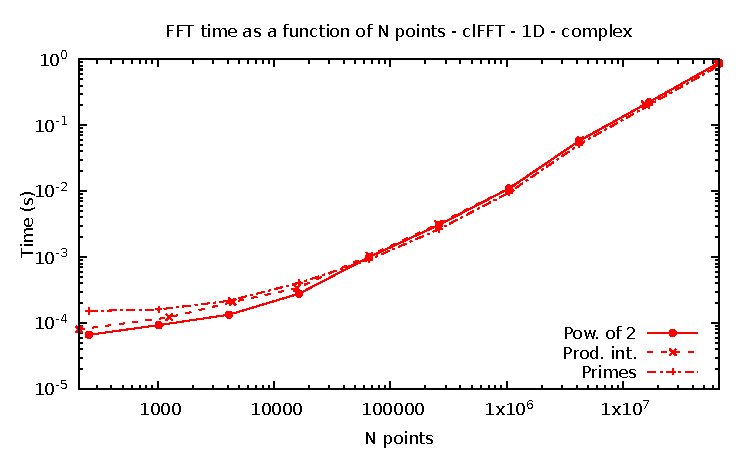
\includegraphics[width=.9\linewidth]{graphs/fft-opencl-1d-pow2-c-exec.pdf}
\caption{Execution (complex)}
\label{FFTCL1DCE}
\end{subfigure}
\caption{Initialisation and execution times as a function of the number of points (OpenCL, 1 dimension)}
\label{FFTCL1D}
\end{figure}

\begin{figure}[H]
\captionsetup{width=0.8\linewidth}
\centering
\begin{subfigure}{.5\textwidth}
\centering
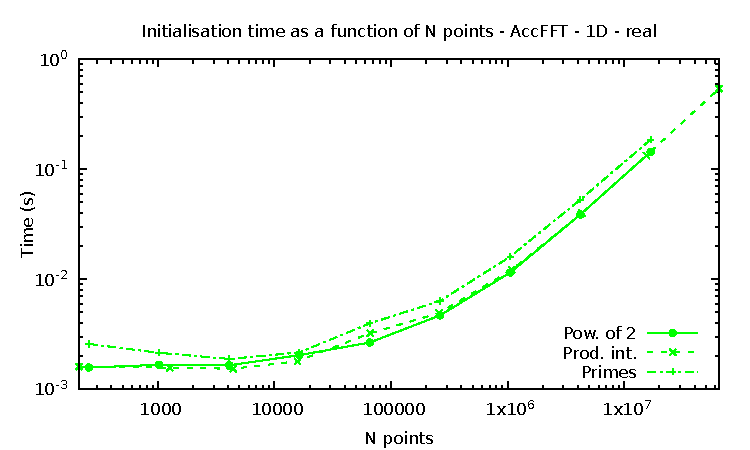
\includegraphics[width=.9\linewidth]{graphs/fft-openacc-1d-pow2-r-init.pdf}
\caption{Intialisation (real)}
\label{FFTACC1DRI}
\end{subfigure}%
\begin{subfigure}{.5\textwidth}
\centering
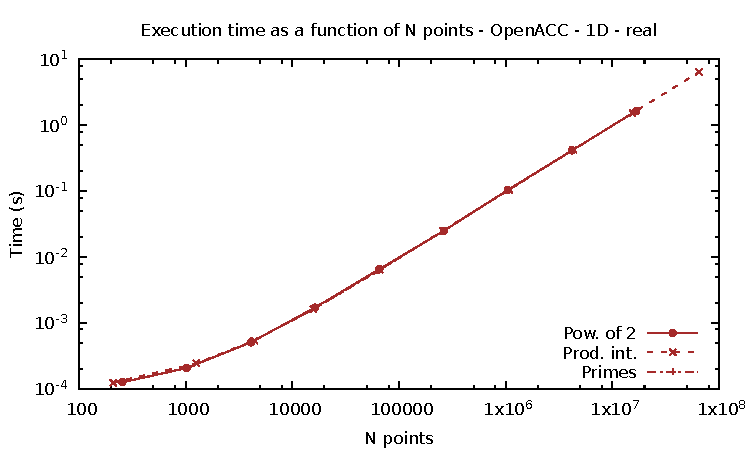
\includegraphics[width=.9\linewidth]{graphs/fft-openacc-1d-pow2-r-exec.pdf}
\caption{Execution (real)}
\label{FFTACC1DRE}
\end{subfigure}\\
\begin{subfigure}{.5\textwidth}
\centering
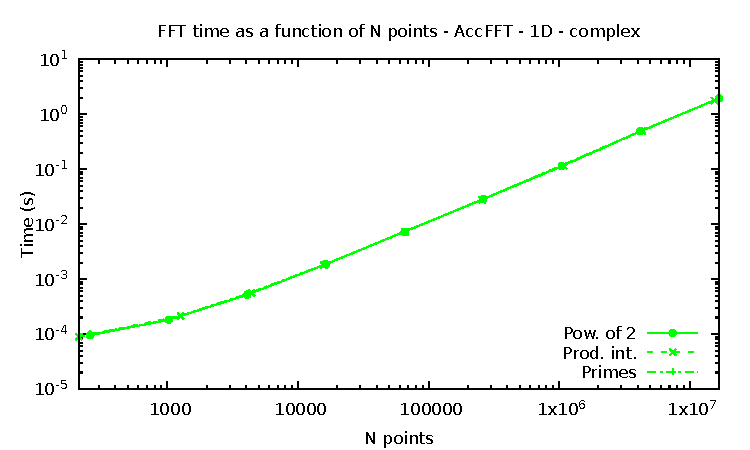
\includegraphics[width=.9\linewidth]{graphs/fft-openacc-1d-pow2-c-exec.pdf}
\caption{Intialisation (complex)}
\label{FFTACC1DCI}
\end{subfigure}%
\begin{subfigure}{.5\textwidth}
\centering
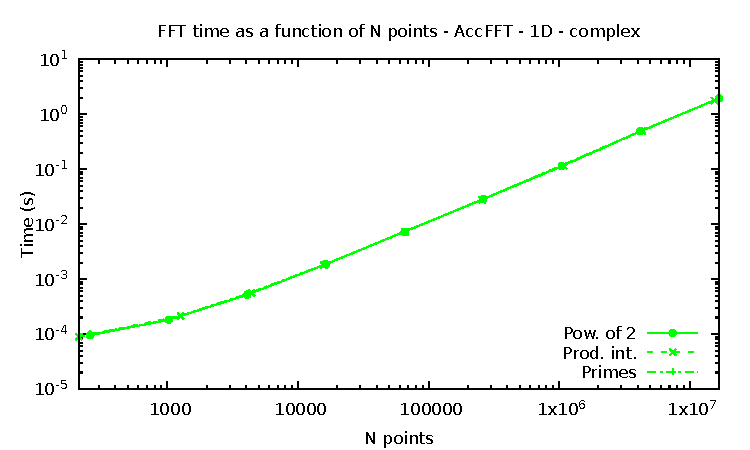
\includegraphics[width=.9\linewidth]{graphs/fft-openacc-1d-pow2-c-exec.pdf}
\caption{Execution (complex)}
\label{FFTACC1DCE}
\end{subfigure}
\caption{Initialisation and execution times as a function of the number of points (OpenACC, 1 dimension)}
\label{FFTACC1D}
\end{figure}


\begin{figure}[H]
\captionsetup{width=0.8\linewidth}
\centering
\begin{subfigure}{.5\textwidth}
\centering
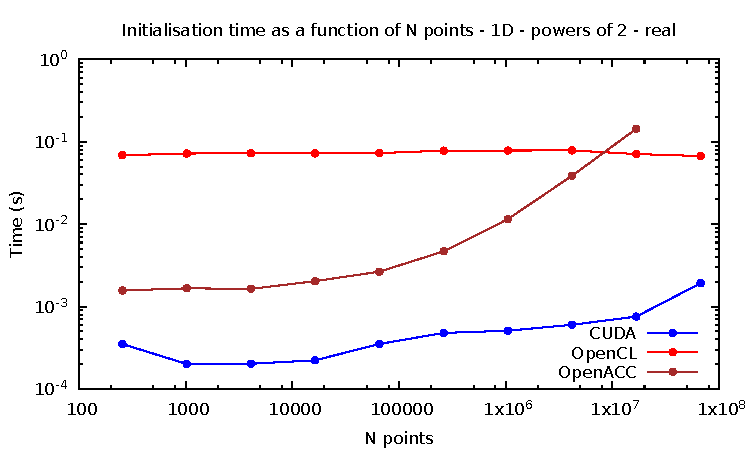
\includegraphics[width=.9\linewidth]{graphs/fft-1d-pow2-r-init.pdf}
\caption{Intialisation (real)}
\label{FFTPOW21DRI}
\end{subfigure}%
\begin{subfigure}{.5\textwidth}
\centering
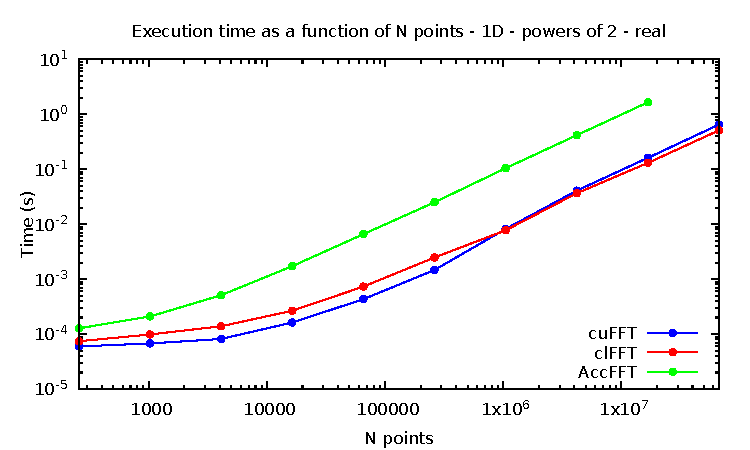
\includegraphics[width=.9\linewidth]{graphs/fft-1d-pow2-r-exec.pdf}
\caption{Execution (real)}
\label{FFTPOW21DRE}
\end{subfigure}\\
\begin{subfigure}{.5\textwidth}
\centering
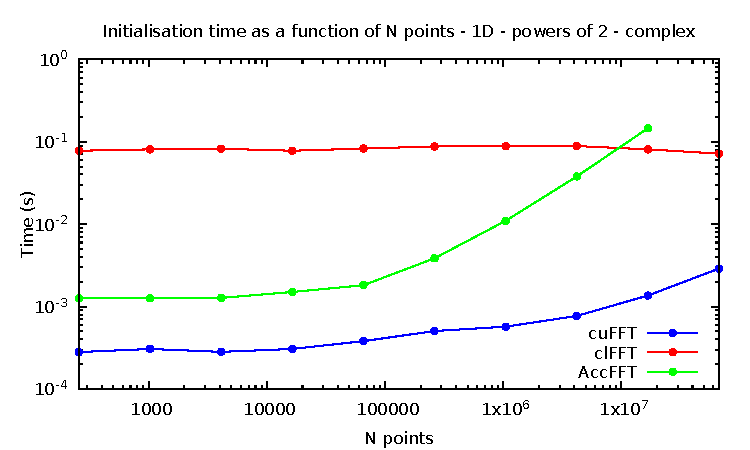
\includegraphics[width=.9\linewidth]{graphs/fft-1d-pow2-c-init.pdf}
\caption{Intialisation (complex)}
\label{FFTPOW21DCI}
\end{subfigure}%
\begin{subfigure}{.5\textwidth}
\centering
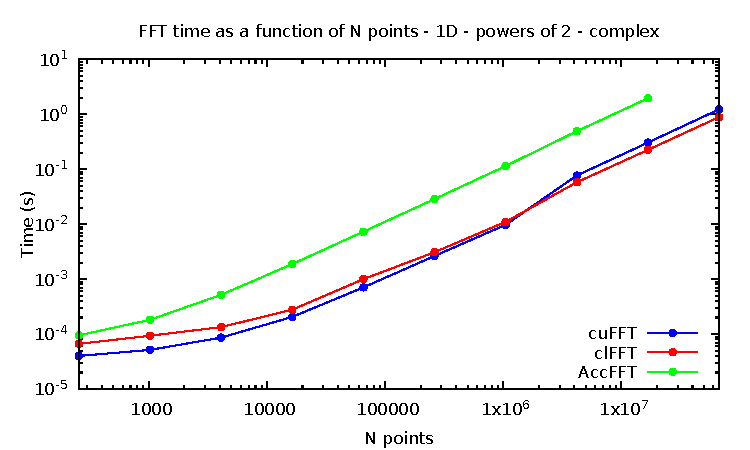
\includegraphics[width=.9\linewidth]{graphs/fft-1d-pow2-c-exec.pdf}
\caption{Execution (complex)}
\label{FFTPOW21DCE}
\end{subfigure}
\caption{Initialisation and execution times as a function of the number of points (1 dimension, powers of 2)}
\label{FFTPOW21D}
\end{figure}


\begin{figure}[H]
\captionsetup{width=0.8\linewidth}
\centering
\begin{subfigure}{.5\textwidth}
\centering
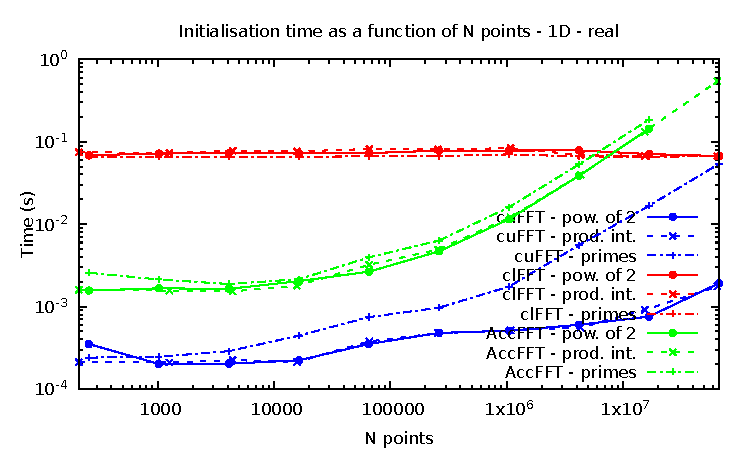
\includegraphics[width=.9\linewidth]{graphs/fft-1d-r-init.pdf}
\caption{Intialisation (real)}
\label{FFT1DRI}
\end{subfigure}%
\begin{subfigure}{.5\textwidth}
\centering
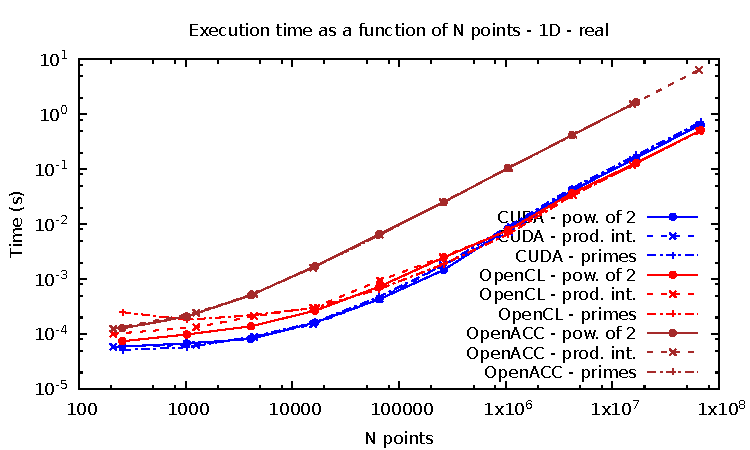
\includegraphics[width=.9\linewidth]{graphs/fft-1d-r-exec.pdf}
\caption{Execution (real)}
\label{FFT1DRE}
\end{subfigure}\\
\begin{subfigure}{.5\textwidth}
\centering
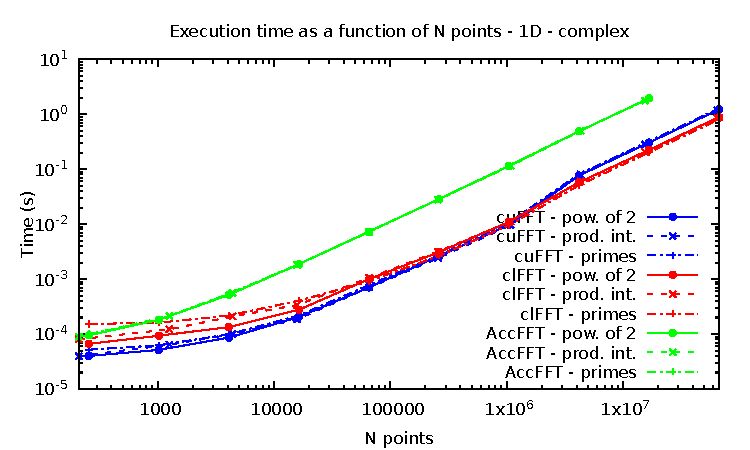
\includegraphics[width=.9\linewidth]{graphs/fft-1d-c-exec.pdf}
\caption{Intialisation (complex)}
\label{FFT1DCI}
\end{subfigure}%
\begin{subfigure}{.5\textwidth}
\centering
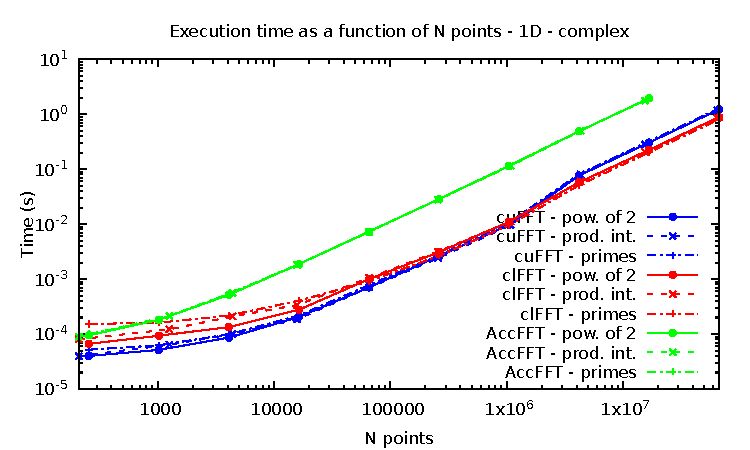
\includegraphics[width=.9\linewidth]{graphs/fft-1d-c-exec.pdf}
\caption{Execution (complex)}
\label{FFT1DCE}
\end{subfigure}
\caption{Initialisation and execution times as a function of the number of points (1 dimension)}
\label{FFT1D}
\end{figure}

\subsection{Effect of the domain size in two dimensions}\label{PERFORMANCE2D}
We repeat the analysis done in Section \ref{PERFORMANCE1D} but, this time, in two dimensions, on a square domain. The sizes of the domain are given in table \ref{2DSIZES}.

\begin{table}[H]
\centering
\begin{tabular}{|l|l|l|}
  \hline
  \multicolumn{3}{|c|}{$N_x=N_y$}\\
  \hline
  \hline
Powers of 2 & prod. pow. int. & primes\\ \hline
$2^9 = 512$ & $2^3\ 3^2\ 7 = 504$ & 509\\ \hline
$2^{10} = 1024$ & $3\ 7^3 = 1029$ & 1021\\ \hline
$2^{11} = 2048$	& $2\ 3 \ 7^3 = 2058$ &	2027\\ \hline
$2^{12} = 4096$	& $2^2\ 3\ 7^3 = 4116$ & 4049\\ \hline
$2^{13} = 8192$	& $2^3\ 3\ 7^3 = 8232$ & 8123\\ \hline
\end{tabular}
\caption{Number of points used for the benchmark in two dimensions}\label{2DSIZES}
\end{table}

In two dimensions, OpenCL performs slightly better than CUDA while OpenACC lags behind. However OpenCL suffers from the same drawback as the one we had identified in Section \ref{PERFORMANCE1D}. In most cases, with CUDA and OpenACC, the performance tends to be worse when the number of points on the side of the domain is a prime number rather than a power of two or the product of powers of small integers. The situation is less clear with OpenCL.

\begin{figure}[H]
\captionsetup{width=0.8\linewidth}
\centering
\begin{subfigure}{.5\textwidth}
\centering
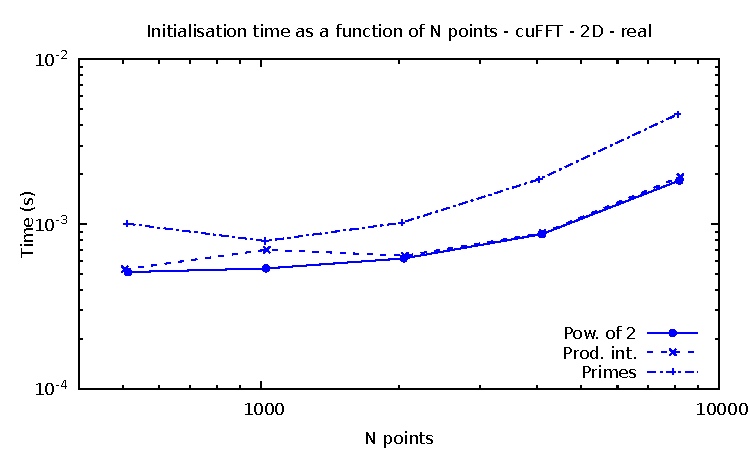
\includegraphics[width=.9\linewidth]{graphs/fft-cuda-2d-pow2-r-init.pdf}
\caption{Intialisation (real)}
\label{FFTCUDA2DRI}
\end{subfigure}%
\begin{subfigure}{.5\textwidth}
\centering
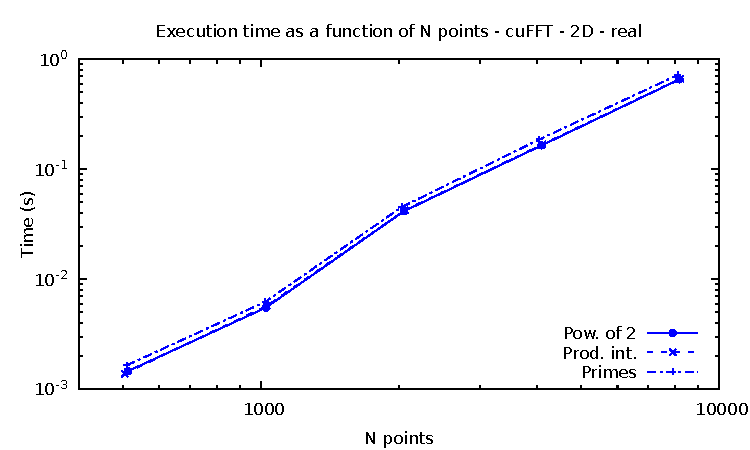
\includegraphics[width=.9\linewidth]{graphs/fft-cuda-2d-pow2-r-exec.pdf}
\caption{Execution (real)}
\label{FFTCUDA2DRE}
\end{subfigure}\\
\begin{subfigure}{.5\textwidth}
\centering
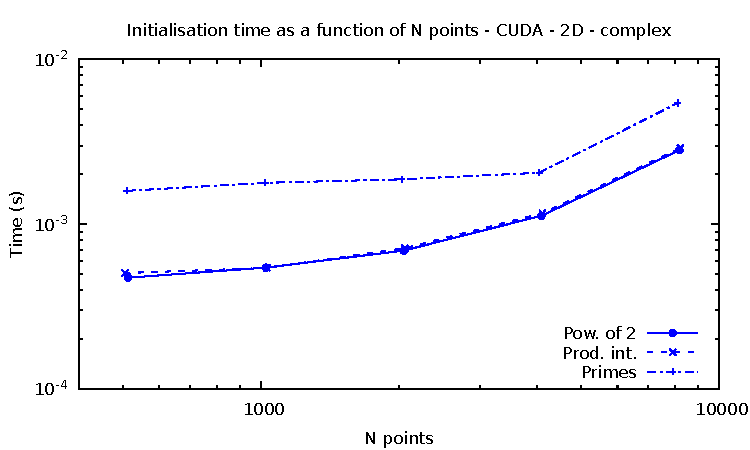
\includegraphics[width=.9\linewidth]{graphs/fft-cuda-2d-pow2-c-init.pdf}
\caption{Intialisation (complex)}
\label{FFTCUDA2DCI}
\end{subfigure}%
\begin{subfigure}{.5\textwidth}
\centering
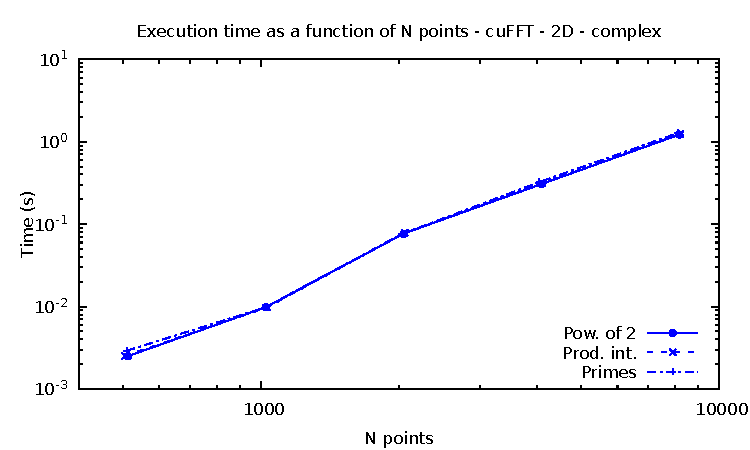
\includegraphics[width=.9\linewidth]{graphs/fft-cuda-2d-pow2-c-exec.pdf}
\caption{Execution (complex)}
\label{FFTCUDA2DCE}
\end{subfigure}
\caption{Initialisation and execution times as a function of the number of points (CUDA, 2 dimensions)}
\label{FFTCUDA2D}
\end{figure}

\begin{figure}[H]
\captionsetup{width=0.8\linewidth}
\centering
\begin{subfigure}{.5\textwidth}
\centering
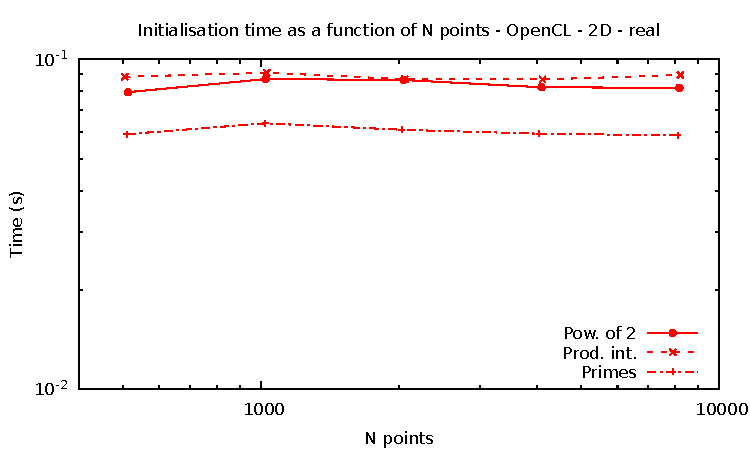
\includegraphics[width=.9\linewidth]{graphs/fft-opencl-2d-pow2-r-init.pdf}
\caption{Intialisation (real)}
\label{FFTCL2DRI}
\end{subfigure}%
\begin{subfigure}{.5\textwidth}
\centering
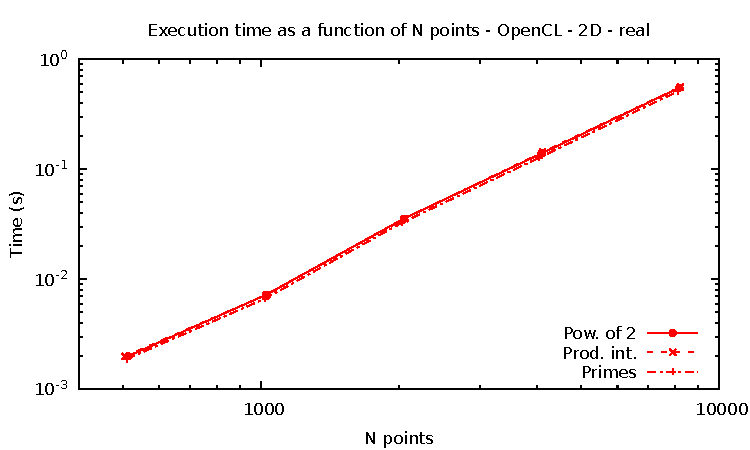
\includegraphics[width=.9\linewidth]{graphs/fft-opencl-2d-pow2-r-exec.pdf}
\caption{Execution (real)}
\label{FFTCL2DRE}
\end{subfigure}\\
\begin{subfigure}{.5\textwidth}
\centering
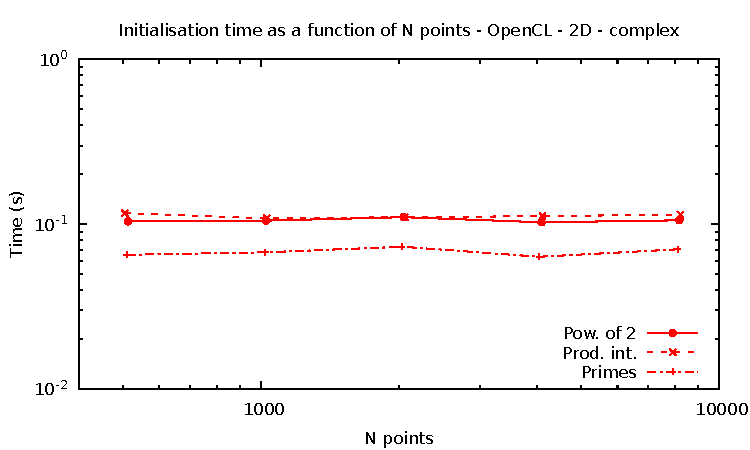
\includegraphics[width=.9\linewidth]{graphs/fft-opencl-2d-pow2-c-init.pdf}
\caption{Intialisation (complex)}
\label{FFTCL2DCI}
\end{subfigure}%
\begin{subfigure}{.5\textwidth}
\centering
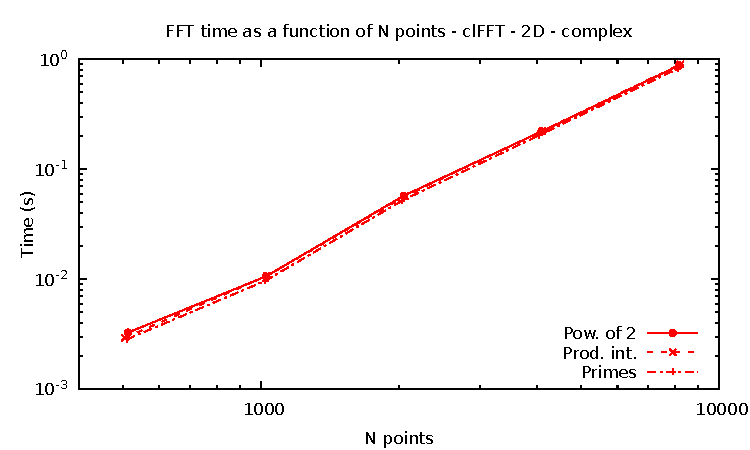
\includegraphics[width=.9\linewidth]{graphs/fft-opencl-2d-pow2-c-exec.pdf}
\caption{Execution (complex)}
\label{FFTCL2DCE}
\end{subfigure}
\caption{Initialisation and execution times as a function of the number of points (OpenCL, 2 dimensions)}
\label{FFTCL2D}
\end{figure}


\begin{figure}[H]
\captionsetup{width=0.8\linewidth}
\centering
\begin{subfigure}{.5\textwidth}
\centering
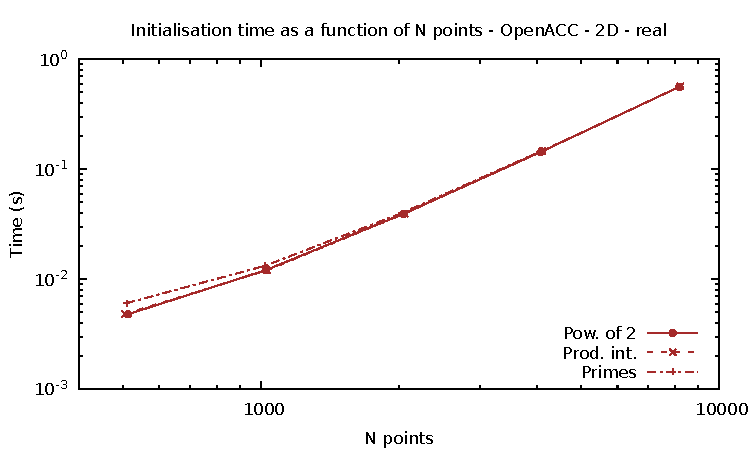
\includegraphics[width=.9\linewidth]{graphs/fft-openacc-2d-pow2-r-init.pdf}
\caption{Intialisation (real)}
\label{FFTACC2DRI}
\end{subfigure}%
\begin{subfigure}{.5\textwidth}
\centering
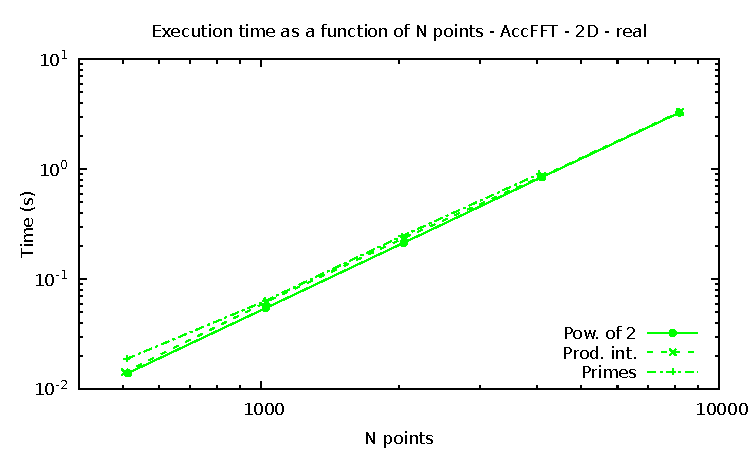
\includegraphics[width=.9\linewidth]{graphs/fft-openacc-2d-pow2-r-exec.pdf}
\caption{Execution (real)}
\label{FFTACC2DRE}
\end{subfigure}\\
\begin{subfigure}{.5\textwidth}
\centering
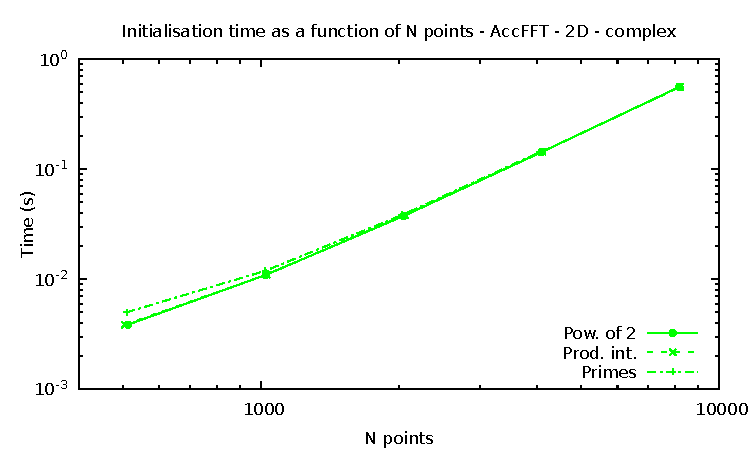
\includegraphics[width=.9\linewidth]{graphs/fft-openacc-2d-pow2-c-init.pdf}
\caption{Intialisation (complex)}
\label{FFTACC2DCI}
\end{subfigure}%
\begin{subfigure}{.5\textwidth}
\centering
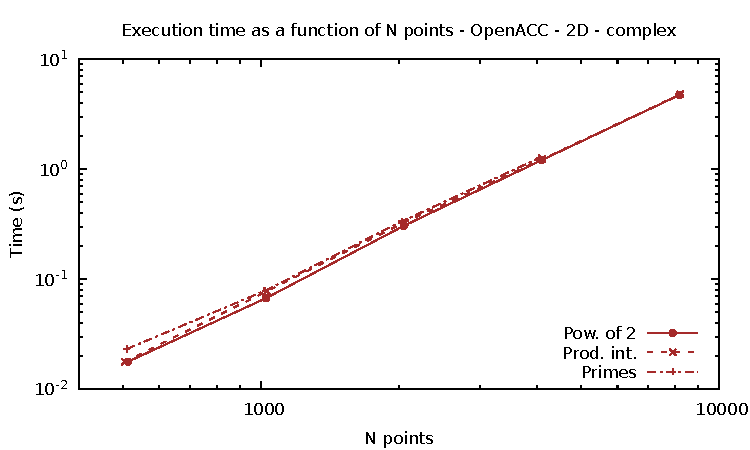
\includegraphics[width=.9\linewidth]{graphs/fft-openacc-2d-pow2-c-exec.pdf}
\caption{Execution (complex)}
\label{FFTACC2DCE}
\end{subfigure}
\caption{Initialisation and execution times as a function of the number of points (OpenACC, 2 dimensions)}
\label{FFTCL2D}
\end{figure}

\begin{figure}[H]
\captionsetup{width=0.8\linewidth}
\centering
\begin{subfigure}{.5\textwidth}
\centering
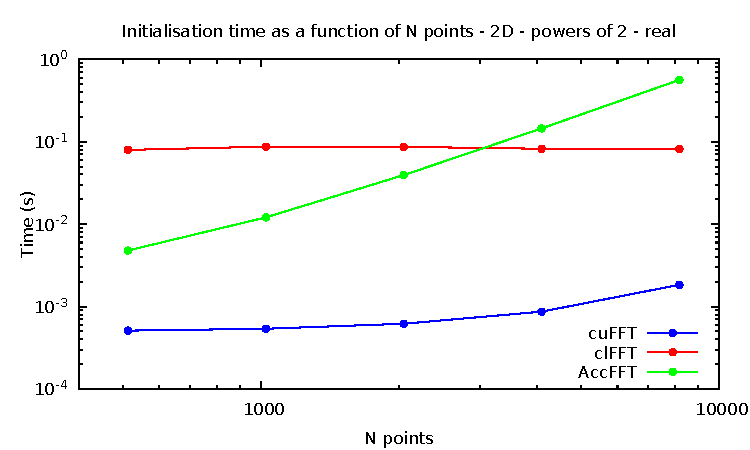
\includegraphics[width=.9\linewidth]{graphs/fft-2d-pow2-r-init.pdf}
\caption{Intialisation (real)}
\label{FFTPOW22DRI}
\end{subfigure}%
\begin{subfigure}{.5\textwidth}
\centering
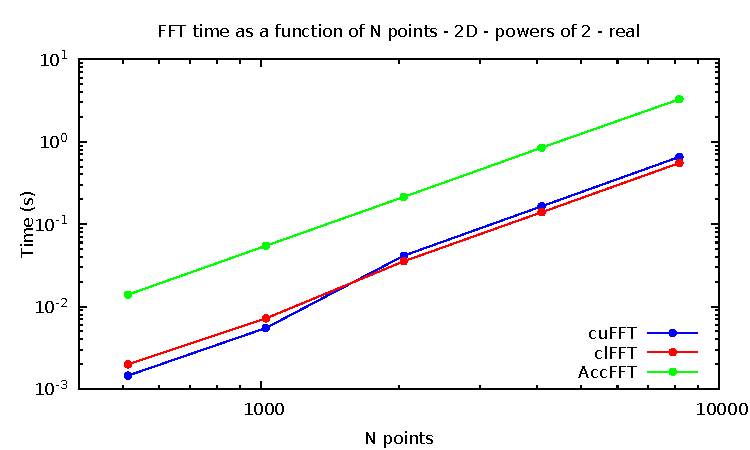
\includegraphics[width=.9\linewidth]{graphs/fft-2d-pow2-r-exec.pdf}
\caption{Execution (real)}
\label{FFTPOW22DRE}
\end{subfigure}\\
\begin{subfigure}{.5\textwidth}
\centering
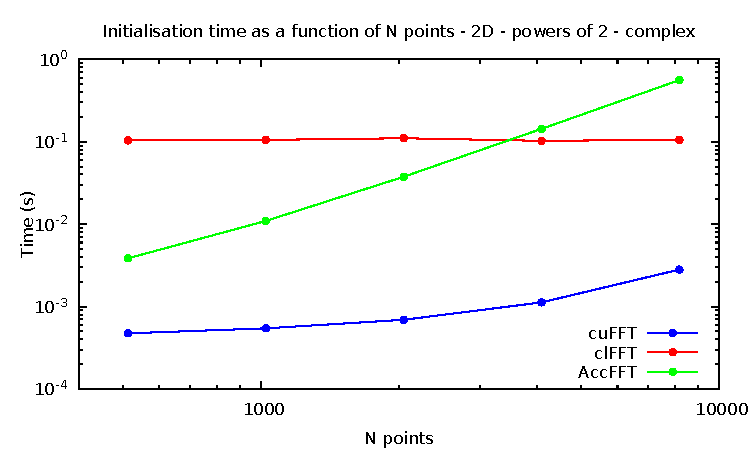
\includegraphics[width=.9\linewidth]{graphs/fft-2d-pow2-c-init.pdf}
\caption{Intialisation (complex)}
\label{FFTPOW22DCI}
\end{subfigure}%
\begin{subfigure}{.5\textwidth}
\centering
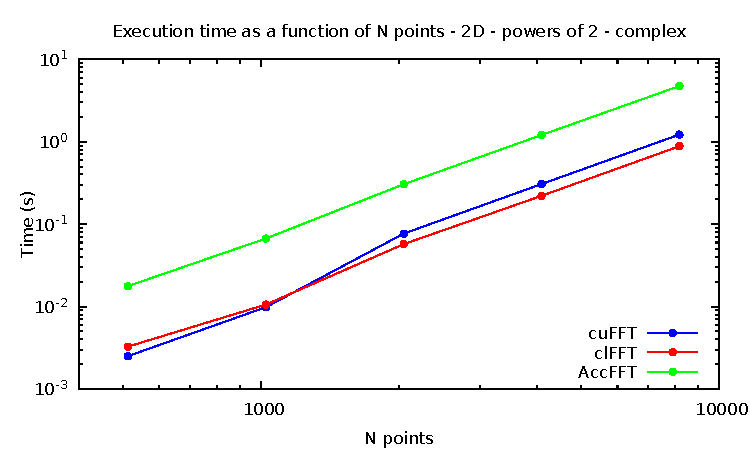
\includegraphics[width=.9\linewidth]{graphs/fft-2d-pow2-c-exec.pdf}
\caption{Execution (complex)}
\label{FFTPOW22DCE}
\end{subfigure}
\caption{Initialisation and execution times as a function of the number of points (2 dimensions, powers of 2)}
\label{FFTPOW22D}
\end{figure}

\begin{figure}[H]
\captionsetup{width=0.8\linewidth}
\centering
\begin{subfigure}{.5\textwidth}
\centering
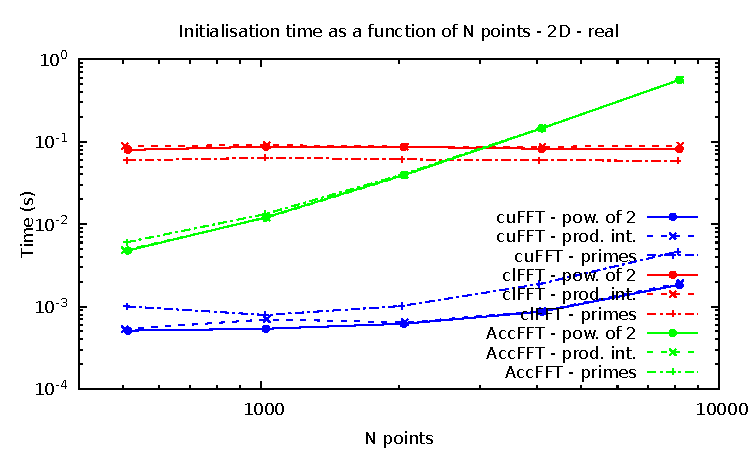
\includegraphics[width=.9\linewidth]{graphs/fft-2d-r-init.pdf}
\caption{Intialisation (real)}
\label{FFT2DRI}
\end{subfigure}%
\begin{subfigure}{.5\textwidth}
\centering
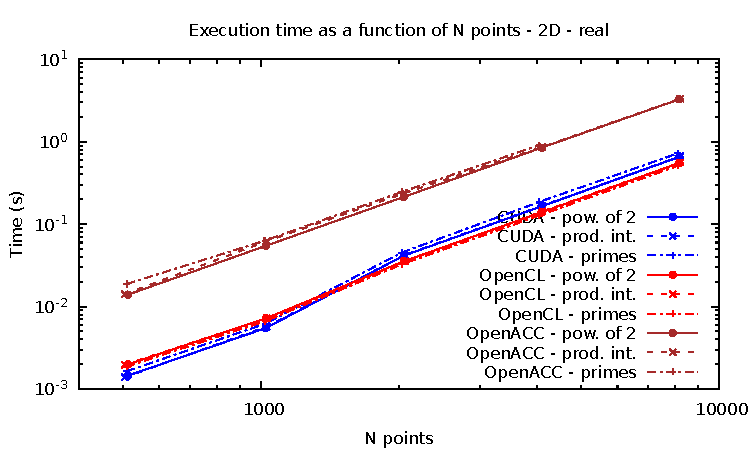
\includegraphics[width=.9\linewidth]{graphs/fft-2d-r-exec.pdf}
\caption{Execution (real)}
\label{FFT2DRE}
\end{subfigure}\\
\begin{subfigure}{.5\textwidth}
\centering
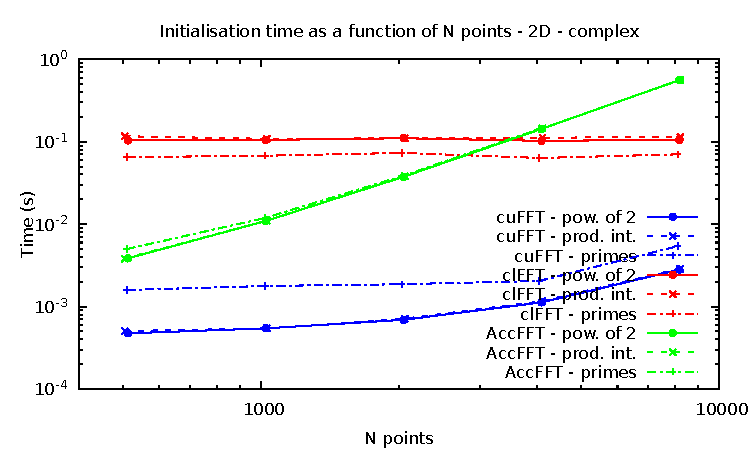
\includegraphics[width=.9\linewidth]{graphs/fft-2d-c-init.pdf}
\caption{Intialisation (complex)}
\label{FFT2DCI}
\end{subfigure}%
\begin{subfigure}{.5\textwidth}
\centering
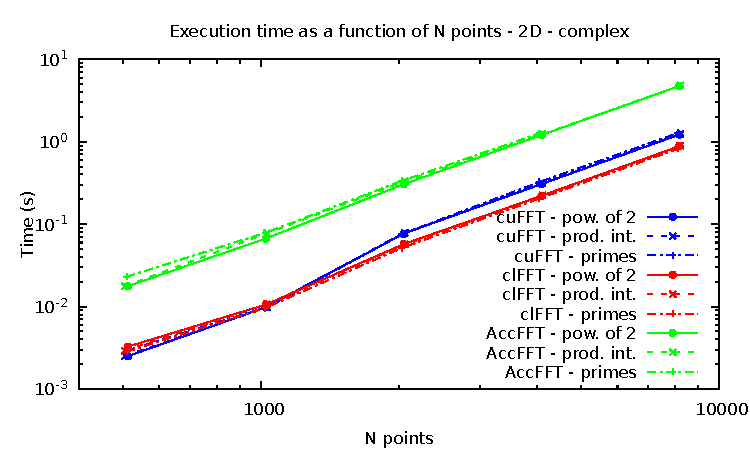
\includegraphics[width=.9\linewidth]{graphs/fft-2d-c-exec.pdf}
\caption{Execution (complex)}
\label{FFT2DCE}
\end{subfigure}
\caption{Initialisation and execution times as a function of the number of points (2 dimensions)}
\label{FFT2D}
\end{figure}


\subsection{Effect of the domain size in three dimensions}\label{PERFORMANCE3D}
After having assessed the performance obtained in one (Section \ref{PERFORMANCE1D}) and two (Section \ref{PERFORMANCE3D}) dimensions, we measure it in three dimensions, on a cubic domain whose sizes are given in Table \ref{3DSIZES}.

\begin{table}[H]
  \centering
  \captionsetup{width=0.8\linewidth}
\begin{tabular}{|l|l|l|}
  \hline
  \multicolumn{3}{|c|}{$N_x=N_y=N_z$}\\
  \hline
  \hline
Powers of 2 & prod. pow. int. & primes\\ \hline
$2^5 = 32$ & $2\ 3\ 5 =	30$ & 31\\ \hline
$2^6 = 64$ & $2\ 5\ 7 = 70$ & 61\\ \hline
$2^7 = 128$ & $3\ 5\ 7 = 105$ & 127\\ \hline
$2^8 = 256$ & $2\ 3\ 5\ 7 = 210$ & 257\\ \hline
$2^9 = 512$ & $2^2\ 3\ 5\ 7 = 420$ & 509\\ \hline
\end{tabular}
\caption{Number of points used for the benchmark in three dimensions}\label{3DSIZES}
\end{table}

In three dimensions, OpenCL and CUDA exhibit performances that are close and they are both significantly faster than OpenACC. However, for large domains, OpenCL performs slightly better. Unfortunately, it is plagued by the problem we identified in the previous section. Its initialisation time is quite long and does not decrease with the number of points. Finally we do not observe any large difference between the performance obtained when the sides of the domain are a power of two, the product of powers of small integers or a prime number.

\begin{figure}[H]
\captionsetup{width=0.8\linewidth}
\centering
\begin{subfigure}{.5\textwidth}
\centering
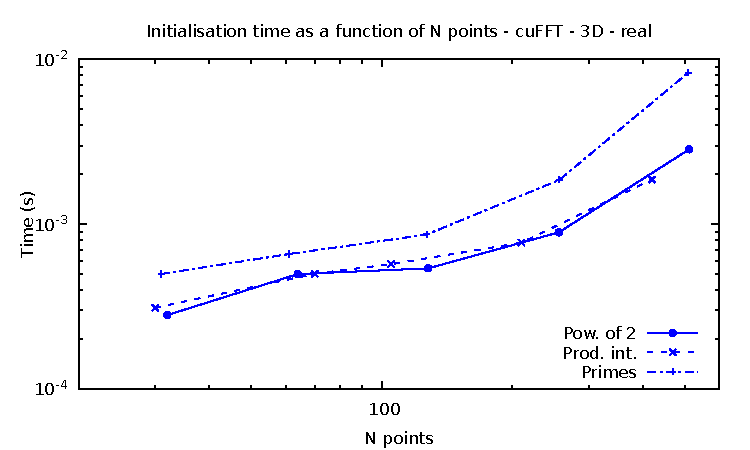
\includegraphics[width=.9\linewidth]{graphs/fft-cuda-3d-pow2-r-init.pdf}
\caption{Intialisation (real)}
\label{FFTCUDA3DRI}
\end{subfigure}%
\begin{subfigure}{.5\textwidth}
\centering
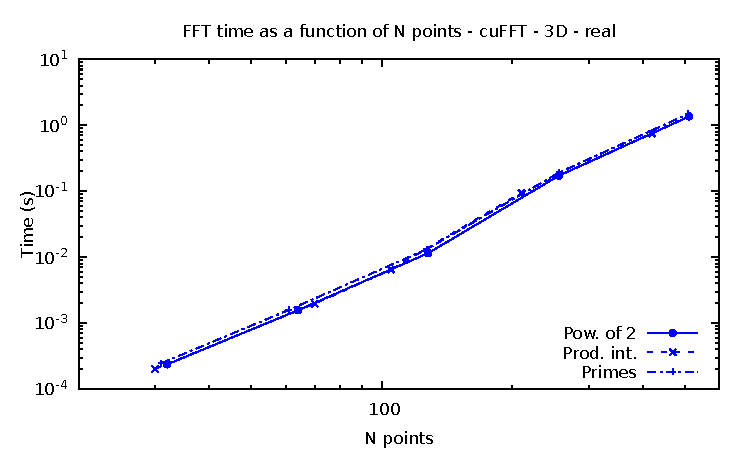
\includegraphics[width=.9\linewidth]{graphs/fft-cuda-3d-pow2-r-exec.pdf}
\caption{Execution (real)}
\label{FFTCUDA3DRE}
\end{subfigure}\\
\begin{subfigure}{.5\textwidth}
\centering
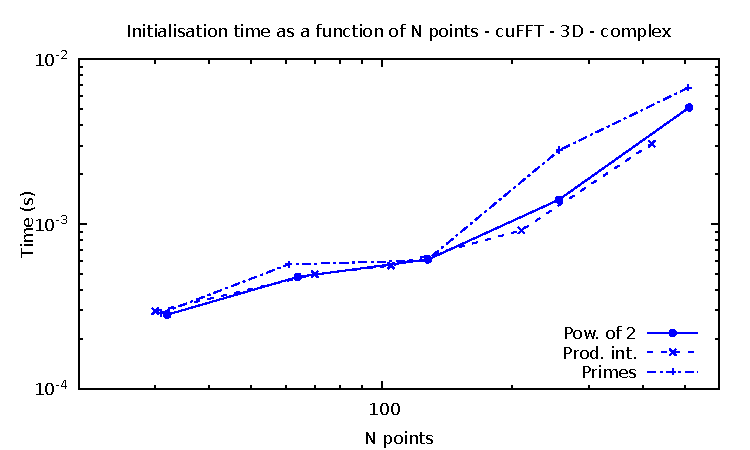
\includegraphics[width=.9\linewidth]{graphs/fft-cuda-3d-pow2-c-init.pdf}
\caption{Intialisation (complex)}
\label{FFTCUDA3DCI}
\end{subfigure}%
\begin{subfigure}{.5\textwidth}
\centering
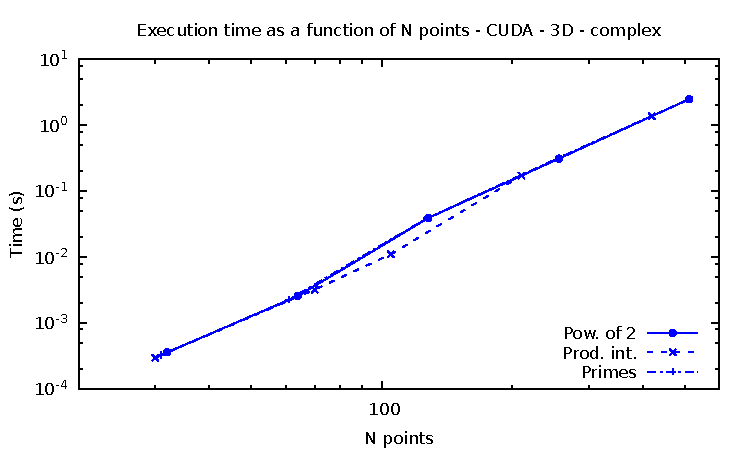
\includegraphics[width=.9\linewidth]{graphs/fft-cuda-3d-pow2-c-exec.pdf}
\caption{Execution (complex)}
\label{FFTCUDA3DCE}
\end{subfigure}
\caption{Initialisation and execution times as a function of the number of points (CUDA, 3 dimensions)}
\label{FFTCUDA3D}
\end{figure}

\begin{figure}[H]
\captionsetup{width=0.8\linewidth}
\centering
\begin{subfigure}{.5\textwidth}
\centering
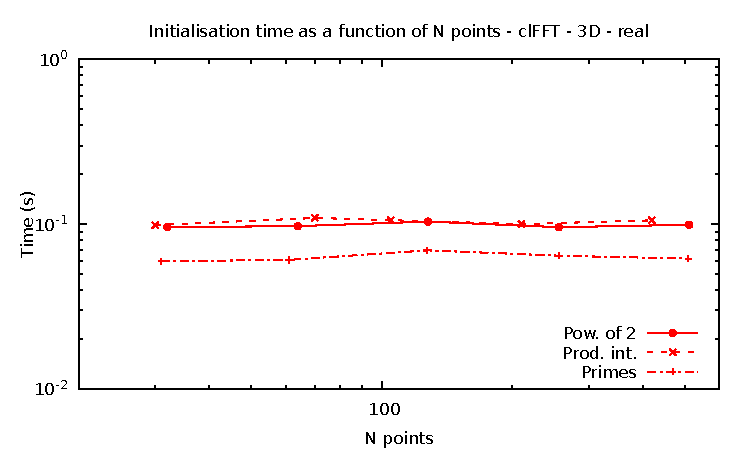
\includegraphics[width=.9\linewidth]{graphs/fft-opencl-3d-pow2-r-init.pdf}
\caption{Intialisation (real)}
\label{FFTCL3DRI}
\end{subfigure}%
\begin{subfigure}{.5\textwidth}
\centering
\includegraphics[width=.9\linewidth]{graphs/fft-opencl-3d-pow2-r-exec.pdf}
\caption{Execution (real)}
\label{FFTCL3DRE}
\end{subfigure}\\
\begin{subfigure}{.5\textwidth}
\centering
\includegraphics[width=.9\linewidth]{graphs/fft-opencl-3d-pow2-c-init.pdf}
\caption{Intialisation (complex)}
\label{FFTCL3DCI}
\end{subfigure}%
\begin{subfigure}{.5\textwidth}
\centering
\includegraphics[width=.9\linewidth]{graphs/fft-opencl-3d-pow2-c-exec.pdf}
\caption{Execution (complex)}
\label{FFTCL3DCE}
\end{subfigure}
\caption{Initialisation and execution times as a function of the number of points (OpenCL, 3 dimensions)}
\label{FFTCL3D}
\end{figure}

\begin{figure}[H]
\captionsetup{width=0.8\linewidth}
\centering
\begin{subfigure}{.5\textwidth}
\centering
\includegraphics[width=.9\linewidth]{graphs/fft-openacc-3d-pow2-r-init.pdf}
\caption{Intialisation (real)}
\label{FFTACC3DRI}
\end{subfigure}%
\begin{subfigure}{.5\textwidth}
\centering
\includegraphics[width=.9\linewidth]{graphs/fft-openacc-3d-pow2-r-exec.pdf}
\caption{Execution (real)}
\label{FFTACC3DRE}
\end{subfigure}\\
\begin{subfigure}{.5\textwidth}
\centering
\includegraphics[width=.9\linewidth]{graphs/fft-openacc-3d-pow2-c-init.pdf}
\caption{Intialisation (complex)}
\label{FFTACC3DCI}
\end{subfigure}%
\begin{subfigure}{.5\textwidth}
\centering
\includegraphics[width=.9\linewidth]{graphs/fft-openacc-3d-pow2-c-exec.pdf}
\caption{Execution (complex)}
\label{FFTACC3DCE}
\end{subfigure}
\caption{Initialisation and execution times as a function of the number of points (OpenACC, 3 dimensions)}
\label{FFTCL3D}
\end{figure}

\begin{figure}[H]
\captionsetup{width=0.8\linewidth}
\centering
\begin{subfigure}{.5\textwidth}
\centering
\includegraphics[width=.9\linewidth]{graphs/fft-3d-pow2-r-init.pdf}
\caption{Intialisation (real)}
\label{FFTPOW23DRI}
\end{subfigure}%
\begin{subfigure}{.5\textwidth}
\centering
\includegraphics[width=.9\linewidth]{graphs/fft-3d-pow2-r-exec.pdf}
\caption{Execution (real)}
\label{FFTPOW23DRE}
\end{subfigure}\\
\begin{subfigure}{.5\textwidth}
\centering
\includegraphics[width=.9\linewidth]{graphs/fft-3d-pow2-c-init.pdf}
\caption{Intialisation (complex)}
\label{FFTPOW23DCI}
\end{subfigure}%
\begin{subfigure}{.5\textwidth}
\centering
\includegraphics[width=.9\linewidth]{graphs/fft-3d-pow2-c-exec.pdf}
\caption{Execution (complex)}
\label{FFTPOW23DCE}
\end{subfigure}
\caption{Initialisation and execution times as a function of the number of points (3 dimensions, powers of 2)}
\label{FFTPOW23D}
\end{figure}

\begin{figure}[H]
\captionsetup{width=0.8\linewidth}
\centering
\begin{subfigure}{.5\textwidth}
\centering
\includegraphics[width=.9\linewidth]{graphs/fft-3d-r-init.pdf}
\caption{Intialisation (real)}
\label{FFT3DRI}
\end{subfigure}%
\begin{subfigure}{.5\textwidth}
\centering
\includegraphics[width=.9\linewidth]{graphs/fft-3d-r-exec.pdf}
\caption{Execution (real)}
\label{FFT3DRE}
\end{subfigure}\\
\begin{subfigure}{.5\textwidth}
\centering
\includegraphics[width=.9\linewidth]{graphs/fft-3d-c-init.pdf}
\caption{Intialisation (complex)}
\label{FFT3DCI}
\end{subfigure}%
\begin{subfigure}{.5\textwidth}
\centering
\includegraphics[width=.9\linewidth]{graphs/fft-3d-c-exec.pdf}
\caption{Execution (complex)}
\label{FFT3DCE}
\end{subfigure}
\caption{Initialisation and execution times as a function of the number of points (3 dimensions)}
\label{FFT3D}
\end{figure}

\subsection{Flatness}\label{FLATNESS}
So far, we have considered only square or cubic domains. In this section, we study the effect of the flatness of the domain by computing the FFT on an increasingly flat cuboid containing $256^3$ points. We define the flatness by the ratio between the number of points in the $z$ and $x$ directions whereas the dimensions in the $x$ and $y$ directions are identical (Flatness:=$N_z/N_x$, $N_x=N_y$) (Table \ref{FLATNESSDIM}). 

\begin{table}[H]
\centering
\begin{tabular}{|l|l|l|}
\hline
$N_x=N_y$ & $N_z $ & Flatness\\ 
\hline
\hline
256 & 256 & 1\\ \hline
128 & 1024 & 8\\ \hline
64 & 4096 & 64\\ \hline
32 & 16384 & 512\\ \hline
16 & 65536 & 4096\\ \hline
8 & 262144 & 32768\\ \hline
4 & 1048576 & 262144\\ \hline 
2 & 4194304 & 2097152\\ \hline
\end{tabular}
\caption{Number of points used for the benchmark in three dimensions}\label{FLATNESSDIM}
\end{table}

We observe that the flatness does not alter significantly the performance which remains dependent only on the total number of points.

\begin{figure}[H]
\captionsetup{width=0.8\linewidth}
\centering
\begin{subfigure}{.5\textwidth}
\centering
\includegraphics[width=.9\linewidth]{graphs/flatness-r-init.pdf}
\caption{Intialisation (real)}
\label{FFT1DRI}
\end{subfigure}%
\begin{subfigure}{.5\textwidth}
\centering
\includegraphics[width=.9\linewidth]{graphs/flatness-r-exec.pdf}
\caption{Execution (real)}
\label{FFT1DRE}
\end{subfigure}\\
\begin{subfigure}{.5\textwidth}
\centering
\includegraphics[width=.9\linewidth]{graphs/flatness-c-init.pdf}
\caption{Intialisation (complex)}
\label{FFT1DCI}
\end{subfigure}%
\begin{subfigure}{.5\textwidth}
\centering
\includegraphics[width=.9\linewidth]{graphs/flatness-c-exec.pdf}
\caption{Execution (complex)}
\label{FFT1DCE}
\end{subfigure}
\caption{Initialisation and execution times as a function of the flatness ($N_z/N_x$, $N_x=N_y$) of the domain (3 dimensions)}
\label{FLATNESSGRAPH}
\end{figure}
\subsection{Requirements from the CCP}\label{CCPPETMR}
We have also benchmarked the libraries provided by these frameworks for the computation of FFTs in a context similar to the situation encountered by the CCP/PET-MR collaboration. In this example, we compute the FFT of 32 square complex images. Their side is made of 252, 256 and 257 points in the cases, respectively, of a number of points corresponding to a product of powers of small integers, a power of 2 or a prime number. In this context, it is CUDA that is the most efficient.
\begin{figure}[H]
\captionsetup{width=0.8\linewidth}
\centering
\begin{subfigure}{.5\textwidth}
\centering
\includegraphics[width=.9\linewidth]{graphs/fft-ccppetmr-init.pdf}
\caption{Intialisation (real)}
\label{FFT1DRI}
\end{subfigure}%
\begin{subfigure}{.5\textwidth}
\centering
\includegraphics[width=.9\linewidth]{graphs/fft-ccppetmr-exec.pdf}
\caption{Execution (real)}
\label{FFT1DRE}
\end{subfigure}
\caption{Initialisation and execution times as a function of the number of points (3 dimensions)}
\label{CCPPETMRGRAPH}
\end{figure}

\section{Conclusion}
For the execution on the GPU of a small piece of code we have programmed, OpenMP was the most efficient framework. In the case of the computation of a FFT using a library, CUDA and OpenCL offer performances that are close. However OpenCL has a very long initialisation time. As a consequence, the library provided by CUDA seems the most efficient. We also note that frameworks based on preprocessor directives, such as OpenMP and OpenACC, are much easier to use. 

\section{Acknowledgements}
The mysterious sentence that only Barbara knows.

\begin{thebibliography}{9}

\bibitem{cuda}
\hyperlink{https://developer.nvidia.com/cuda-zone}{https://developer.nvidia.com/cuda-zone}

\bibitem{opencl}
\hyperlink{https://www.khronos.org/opencl/}{https://www.khronos.org/opencl/}

\bibitem{openacc}
\hyperlink{https://www.openmp.org/}{https://www.openmp.org/}
  
\bibitem{openmp}
\hyperlink{https://www.openmp.org/}{https://www.openmp.org/}

\bibitem{kokkos}
\hyperlink{https://github.com/kokkos}{https://github.com/kokkos}

\bibitem{cufft}
\hyperlink{https://docs.nvidia.com/cuda/cufft/index.html}{https://docs.nvidia.com/cuda/cufft/index.html}

\bibitem{clfft}
  \hyperlink{https://github.com/clMathLibraries/clFFT}{https://github.com/clMathLibraries/clFFT}
  
\bibitem{accfft}
\hyperlink{http://accfft.org/}{http://accfft.org/}

\bibitem{casa}
McMullin, J. P., Waters, B., Schiebel, D., Young, W., Golap, K.,
{\it Astronomical Data Analysis Software and Systems XVI},
ASP Conf. Ser. 376, ed. R. A. Shaw, F. Hill, D. J. Bell (San Francisco, CA: ASP), 127

\bibitem{FFTREPORT}
The FFT technical report.

\bibitem{ccppetmr}
\hyperlink{https://www.ccppetmr.ac.uk/}{https://www.ccppetmr.ac.uk/}

\bibitem{softwareoutlook}
\hyperlink{https://www.softwareoutlook.ac.uk/}{https://www.softwareoutlook.ac.uk/}

\bibitem{KOKKOSDOC}
\hyperlink{https://github.com/kokkos/kokkos/wiki/Compiling}{https://github.com/kokkos/kokkos/wiki/Compiling}

\end{thebibliography}

\end{document}
